\section{Conclusioni}
\subsection{Conversazione e Mood}
Una parte fondamentale della conversazione che si ha con un assistente è sicuramente il fatto che esso non sia \textbf{statico} nel tempo ma che riesca ad interpretare la situazione e rispondere di conseguenza.
Questo fatto è stato codificato sotto forma di \textbf{emozioni dinamiche}.
\\
Il metodo \texttt{check\_for\_mood\_change} ci restituisce, data la situazione corrente del nostro frame, l'emozione corretta da includere nel nostro assistente personale. L'emozione cambia totalmente il corpus utilizzato da Piton, i voti che ci può dare e la quantità di errori che possiamo effettuare prima che l'interazione non si interrompa.
\subsubsection{Da angry ad happy}
In questo primo caso possiamo notare dall'immagine \ref{fig:from_angry_to_happy} come un'interazione perfetta può trasformare anche l'emozione più bassa (angry) nella più alta (happy). Dallo stato angry, però, non potrà passare direttamente ad happy, ma dovrà essere un passaggio graduale, giusto per non renderlo esattamente uno \textit{psicopatico} (un normale umano, se non in rari casi, non passa immediatamente dalla rabbia alla gioia).
\subsubsection{Da happy ad angry}
In questo secondo caso, presentato nell'immagine \ref{fig:from_happy_to_angry} cerchiamo di far passare Piton dall'essere felice ad essere arrabbiato: l'unica maniera ovviamente è quella di sbagliare la maggior parte delle domande e di portare l'interazione ad avere quanti più turni possibili.
\subsubsection{Un fallimento totale}
Come già citato in \ref{sec:3} il discorso termina immediatamente con un fallimento nel qual caso lo studente non sappia rispondere ad una domanda e lo affermi esplicitamente \ref{fig:a_complete_failure}.
\subsection{Possibili miglioramenti}
\subsubsection{Nell'analisi del discorso}
Il nostro sistema di dialogo è in grado di esaminare ed elaborare un ampio set di tipologie di risposte, domande, frasi non utili; è comunque possibile approfondire in merito e integrare tutte le possibili tipologie di risposte che un utente può porre.
\subsubsection{Nella generazione del linguaggio}
Come spiegato nei paragrafi precedenti la generazione del linguaggio avviene tramite catene di Markov, è stata già discusso il problema delle possibili frasi prive di senso o comunque non utili al nostro scopo. Può essere sicuramente utile ampliare la lista di frasi utilizzate per la generazione. Ma una possibile soluzione definitiva può essere quella di utilizzare dei \textbf{transformer} come gpt3 per generare domande e frasi filler sempre corrette e coerenti.

\subsubsection{Migliore Usabilità}
L'interazione con terminale può risultare scomoda, soprattutto per persone fuori dal mondo informatico. Per migliorare l'usabilità del progetto si dovrebbe quindi usare un sistema di \textit{Automatic Speech Recognition} per riconoscere il parlato ed uno di \textit{Text-To-Speech} per dar voce al professore e rendere il dialogo il più umano possibile.
\subsection{Immagini Interazione}
\begin{figure}[!hp]
    \centering
    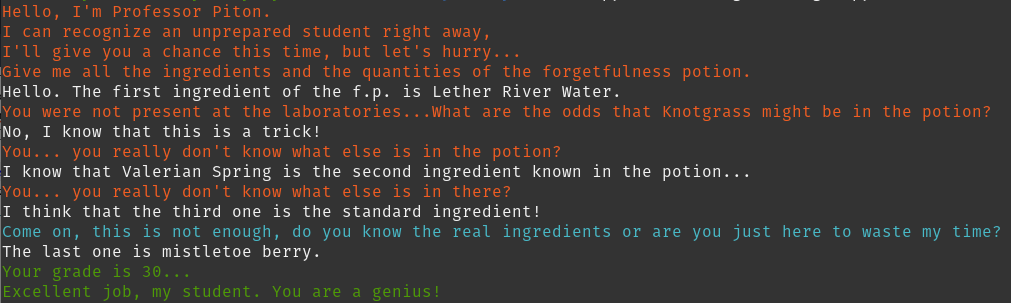
\includegraphics[scale=0.37]{Images/from_angry_to_happy.png}
    \caption{Interazione perfetta tra un Piton angry ed un ottimo studente}
    \label{fig:from_angry_to_happy}
\end{figure}
\begin{figure}[!hp]
    \centering
    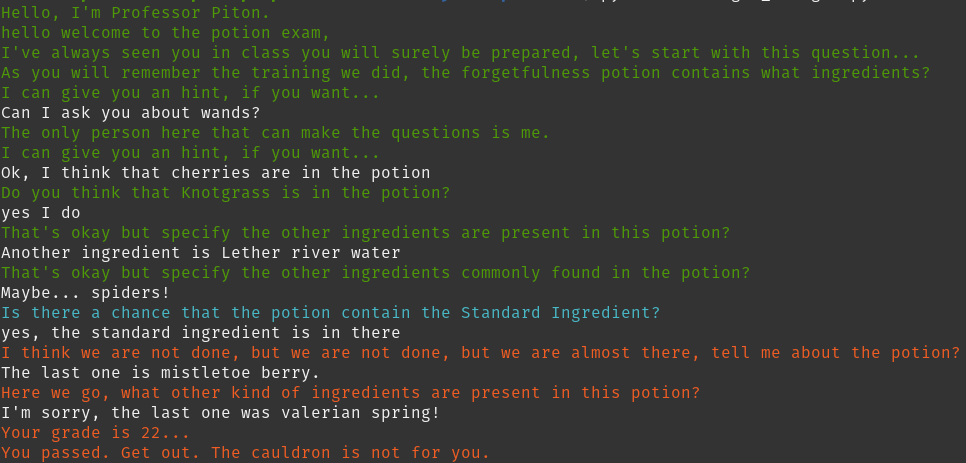
\includegraphics[scale=0.4]{Images/from_happy_to_angry.png}
    \caption{L'utente non sa molto: Piton passa velocemente da essere felice ad arrabbiato}
    \label{fig:from_happy_to_angry}
\end{figure}
\begin{figure}[!hp]
    \centering
    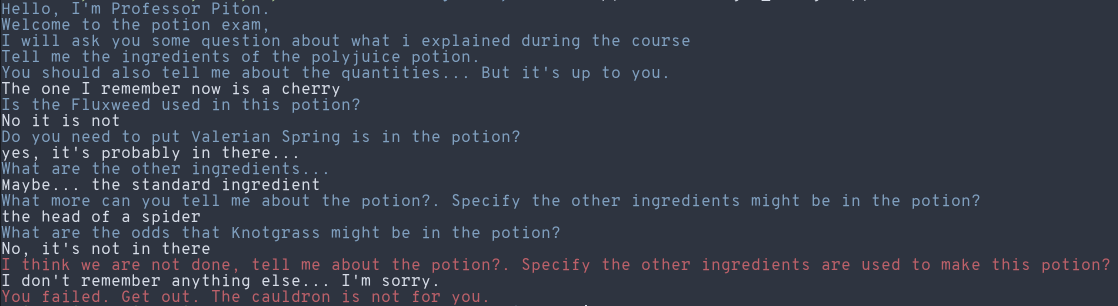
\includegraphics[scale=0.37]{Images/a_complete_fail.png}
    \caption{Un fallimento totale da parte dell'utente. Ogni risposta è errata.}
    \label{fig:a_complete_failure}
\end{figure}